\section{Enterprise Resource Planning}

Enterprise Resource Planning (ERP) systems often feature vertical solutions specifically designed to meet the needs of different industries. 
These solutions are tailored to be highly specialized.
However, we can make a broader distinction between manufacturing and service companies:
\begin{itemize}
    \item Manufacturing companies produce tangible products.
    \item Service companies provide intangible products.
\end{itemize}
\noindent 
Companies typically rely on three main IT functional portfolios within their ERP systems: administrative, operational, and executive. 
These portfolios, while initially developed separately, are now integrated within modern ERP systems, forming the core functionalities of these systems.

\begin{figure}[H]
    \centering
    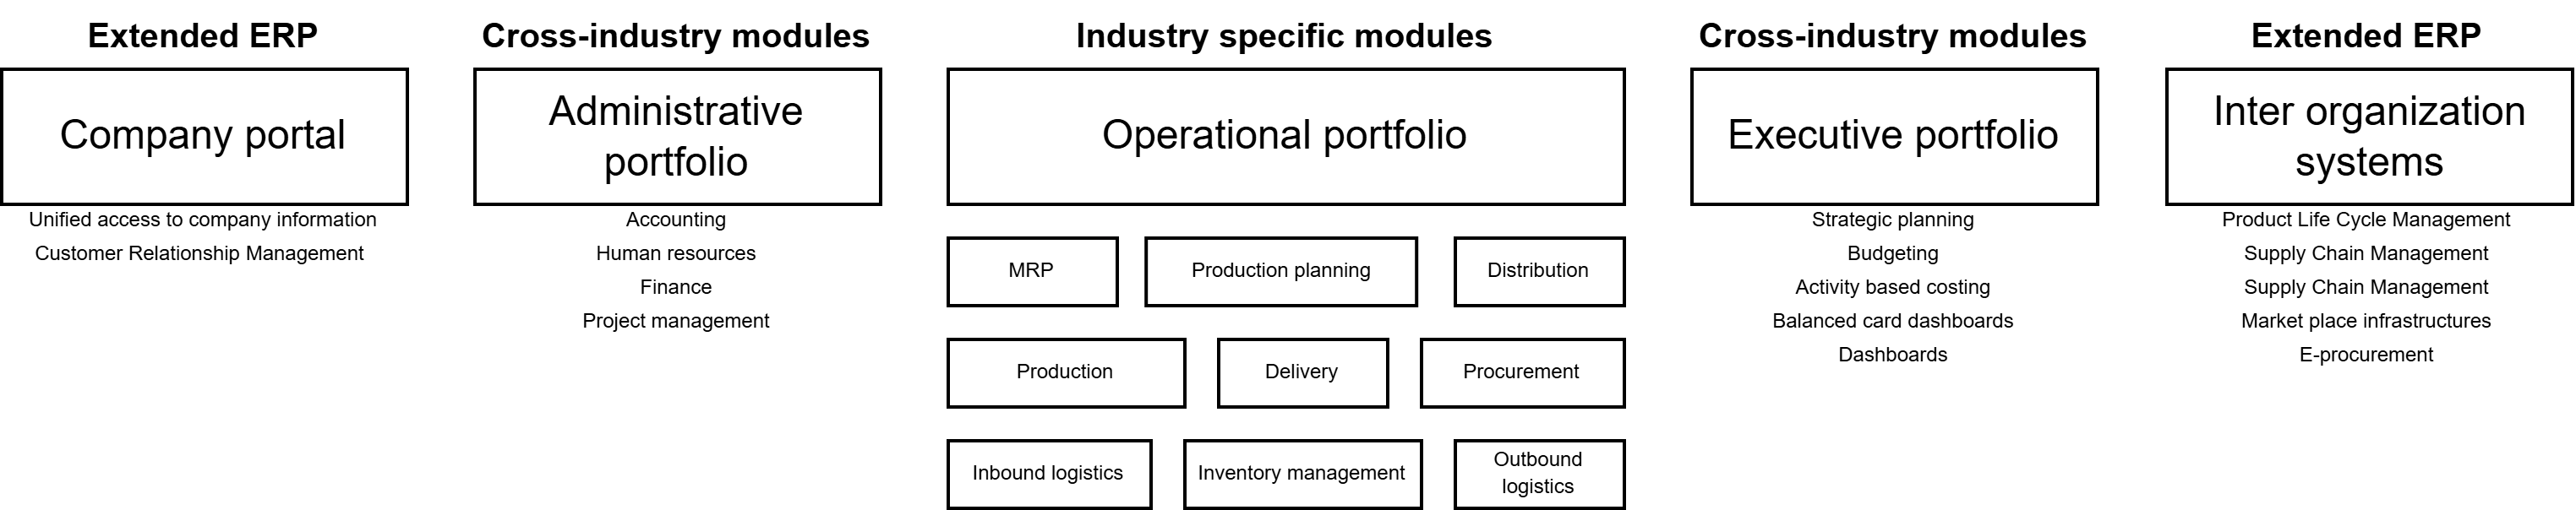
\includegraphics[width=1\linewidth]{images/bis1.png}
    \caption{ERP architecture}
\end{figure}